\documentclass{article}

% if you need to pass options to natbib, use, e.g.:
%     \PassOptionsToPackage{numbers, compress}{natbib}
% before loading neurips_2018

% ready for submission
%     \usepackage{neurips_2018}

% to compile a preprint version, e.g., for submission to arXiv, add add the
% [preprint] option:
%     \usepackage[preprint]{neurips_2018}

% to compile a camera-ready version, add the [final] option, e.g.:
\usepackage[final]{neurips_2018}

% to avoid loading the natbib package, add option nonatbib:
%     \usepackage[nonatbib]{neurips_2018}

\usepackage[utf8]{inputenc} % allow utf-8 input
\usepackage[T1]{fontenc}    % use 8-bit T1 fonts
\usepackage{hyperref}       % hyperlinks
\usepackage{url}            % simple URL typesetting
\usepackage{booktabs}       % professional-quality tables
\usepackage{amsfonts}       % blackboard math symbols
\usepackage{nicefrac}       % compact symbols for 1/2, etc.
\usepackage{microtype}      % microtypography
\usepackage[T2A]{fontenc}
\usepackage[utf8]{inputenc}
\usepackage[english, russian]{babel}
\usepackage{graphicx}

\title{Learning to Infer Graphics Programs from Hand-Drawn Images}

% The \author macro works with any number of authors. There are two commands
% used to separate the names and addresses of multiple authors: \And and \AND.
%
% Using \And between authors leaves it to LaTeX to determine where to break the
% lines. Using \AND forces a line break at that point. So, if LaTeX puts 3 of 4
% authors names on the first line, and the last on the second line, try using
% \AND instead of \And before the third author name.

\author{%
  Mikhailov Nikita M.\\
  Faculty of Computer Science\\
  Highter School of Economics\\
  Moscow\\
  \texttt{nmmikhaylov@edu.hse.ru} \\
  % examples of more authors
  % \And
  % Coauthor \\
  % Affiliation \\
  % Address \\
  % \texttt{email} \\
  % \AND
  % Coauthor \\
  % Affiliation \\
  % Address \\
  % \texttt{email} \\
  % \And
  % Coauthor \\
  % Affiliation \\
  % Address \\
  % \texttt{email} \\
  % \And
  % Coauthor \\
  % Affiliation \\
  % Address \\
  % \texttt{email} \\
}

\begin{document}
% \nipsfinalcopy is no longer used

\maketitle

\begin{abstract}
  Это промужуточный отчет проекта по воспроизведению статьи 
  \begin{center}
      \href{https://arxiv.org/pdf/1707.09627.pdf}{Learning to Infer Graphics Programs from Hand-Drawn Images}
  \end{center}
  В рамках требований к промежуточномой контрольной точке тут выполнен разбор используемого в работе DSL, реализован работающий модуль для рендера, а так же модуль генерации данных
  \begin{center}
      \href{https://github.com/Mikhail-off/Hand-Drawn-Images-Recognition}{Ссылка на GitHub проекта}
  \end{center}
\end{abstract}

\section{Описание задачи}
Часто мы нуждаемся в различных диаграммах. Для этого мы пользуемся различными инструментами для их создания. На каждую такую картинку мы тратим время, а хотелось бы просто от руки схематично нарисовать, чтобы потом программа сама все выравняла, соединила нужные точки (например, чтобы два круга, центры которых на одной прямой, были соединены ровно по этой прямой). Этим и вдохновились авторы статьи.\\
Сама задача состоит в том, чтобы по нарисованным от руки картинкам выдавать
\begin{enumerate}
    \item Программу, с помощью которой можно эту диаграмму создать
    \item Изображение, построенное на основе программы. В идеале ровную картинку со входа
\end{enumerate}
Мы работаем с диаграммами, а они часто состоят из простых объектов, например, прямоугольников, окружностей, отрезков. Отступим от такой классической схемы лишь в отрезках: добавим им возможность быть направленными -- со стрелочкой, и быть пунктирной. \\
Авторы статьи назвали эту задачу <<Program Learning>>. Так же мы не хотим выдавать простой набор команд, например:
\begin{enumerate}
    \item Прямоугольник с точками $(1, 1), (2, 2)$
    \item Прямоугольник с точками $(2, 2), (3, 3)$
    \item Прямоугольник с точками $(3, 3), (4, 4)$
    \item Прямоугольник с точками $(4, 4), (5, 5)$
\end{enumerate}
Очевидно, такие прямоугольники можно нарисовать циклом:
\begin{enumerate}
    \item[] Цикл по $i \in [1, 4]$:
    \item[] \qquad Прямоугольник с точками $(i, i), (i + 1, i + 1)$
\end{enumerate}
После того, как мы выяснили, какие объекты должны быть на сцене, мы должны выдать оптимальную с некоторой точки зрения программу для их рендеринга.

\section{Подход к решению задачи}
Предсказывать все объекты целиком слишком сложно, поэтому авторы статьи предлагают действовать итерационно. Пусть у нас есть входное изображение $S(ource)$ и изображение $R(endered)$, полученное после рендера. Изначально $R$ -- пустое:
\begin{enumerate}
    \item Подаем на вход сети двухканальное изображение $[S, R]$
    \item Сеть сравнивает $S$ и $R$ и решает, какой объект рисовать дальше. То есть выдает объект $O$
    \item Генерируем новое изображение $R$ уже с объектом $O$. 
    \item Возвращаемся к п.1, пока $O \neq END$
\end{enumerate}
\begin{center}
    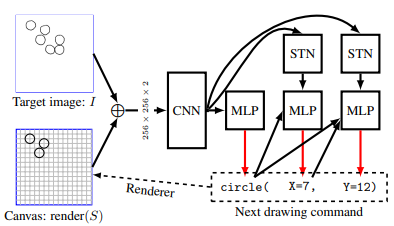
\includegraphics[width=100mm]{Images/1.png}
\end{center}

Саму сеть будем проектировать в следующей части проекта. Прежде всего нужно подготовить данные для обучения. Авторы статьи утверждают, что сеть хорошо учится даже на синтетических данных.

\section{Генерация данных}
Генерировать данные будем с помощью \LaTeX, в котором есть TikZ. Диаграмма -- это прежде всего набор различных фигур. Разобьем изображение на сетку размера $16\times16$. Введем описание каждого из объектов:
\begin{enumerate}
    \item Точка. У нее есть координаты $x, y$. Генерировать ее координаты будем с некоторой вероятностью из уже имеющихся точек на сцене, либо случайно из сетки.
    \item Окружность. У нее есть центр -- точка, и радиус. Генерировать ее будем следующим образом: сначала пройдемся по всем существующим окружностям, далее с некоторой вероятностью переиспользуем один из радиусов и сгенерируем центр. Если полученная окружность выходит за рамки сетки, то повторяем заново, пока не получим валидную окружность.
    \item Прямоугольник. У него есть четыре угла -- четыре точки. Задается однозначно лишь по двум противоположным. Семплируем две точки. Одну из них назначаем верхним левым углом, вторую правым нижним (если нужно меняем координаты так, чтобы все было хорошо).
    \item Линия. У нее есть две точки. Самое сложное в плане генерации. На диаграммах линии чаще всего используются, чтобы соединять объекты, поэтому точки для линий мы будем семплировать из специальных точек существующих объектов. Каждый объект имеет точки, которыми его можно присоединить. Генерируем все такие прямые, а далее с некоторой вероятностью выбираем случайную из них, а иначе случайно семплируем две точки линии.
\end{enumerate}

Казалось бы этого достаточно, но мы не учли пересечения объектов. Будем добавлять на текущую сцену объект, только если он не пересекает никакой из уже существующих объектов.\\
Для генерации <<чистых>> данных этого достаточно, однако нам нужно имитировать нарисованные от руки изображения. Для этого каждому объекту добавим шум в координаты и будем использовать атрибут <<pencildraw>>, который делает как раз то, что нам нужно. После этого <<перегоним>> все объекты в \LaTeX программу, скомпилируем $pdf$-файл, сконвертируем изображения оттуда в $png$-картинки. Вот что из этого получилось:
\begin{center}
    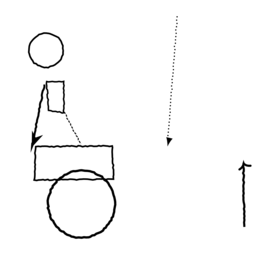
\includegraphics[width=50mm]{Images/2.png}
    \qquad \qquad
    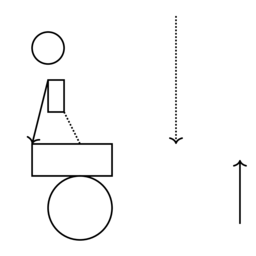
\includegraphics[width=50mm]{Images/2_orig.png}
\end{center}
\begin{center}
    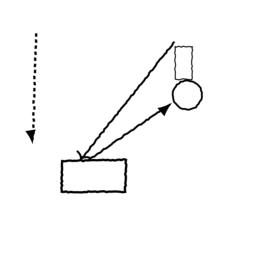
\includegraphics[width=50mm]{Images/3.png}
    \qquad
    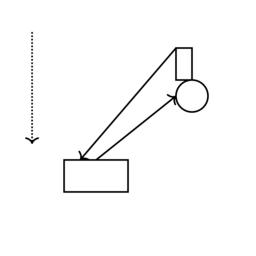
\includegraphics[width=50mm]{Images/3_orig.png}
\end{center}

Слева -- имитация рукописных изображений, справа -- ровное изображение, полученное в результате генерации.
Если посмотреть на оригинальную статью, то синтетические данные у них не лучше, поэтому считаем что мы пришли к успеху и реализовали модуль генерации данных, а так же их рендера. Все же это не диаграммы, но для данных, на которых мы будем обучаться должно подойти. Все такие самое главное -- научиться детектировать объект, отнести его к нужному классу и предсказать его правильные координаты так, чтобы все было ровно.
\newpage

\section{DSL}
Начнем с того, а что вообще такое DSL? Domain-Specific Language(DSL) -- язык программирования специализированный для конкретной области применения. В нашем случае -- для изображения диаграмм. 

Мы разрешаем (\texttt{for}), условия (\texttt{if}), вертикальные/горизонтальные отражения (\texttt{reflect}), переменные (Var) и афинные преобразования ($\mathbb{Z}\times$Var\texttt{+}$\mathbb{Z}$). 
\hbox{
\begin{tabular}{rl}\toprule
  Program$\to$&Statement; $\cdots$; Statement\\
  Statement$\to$&\texttt{circle}(Expression,Expression)\\
  Statement$\to$&\texttt{rectangle}(Expression,Expression,Expression,Expression)\\
  Statement$\to$&\texttt{line}(Expression,Expression,Expression,Expression,Boolean,Boolean)\\
  Statement$\to$&\texttt{for}$(0\leq \text{Var}  < \text{Expression})$\texttt{ \{ if }$(\text{Var} > 0)$\texttt{ \{ }Program\texttt{ \}; }Program\texttt{ \}}\\
  Statement$\to$&\texttt{reflect}$(\text{Axis})$\texttt{ \{ }Program\texttt{ \}}\\
  Expression$\to$&$\mathbb{Z}\times$Var\texttt{+}$\mathbb{Z}$\\
%  Var$\to$&A free (unused) variable\\
  Axis$\to$&\texttt{X = }$\mathbb{Z}$ | \texttt{Y = }$\mathbb{Z}$\\
    $\mathbb{Z}\to$&an integer\\\bottomrule
  \end{tabular}
}
\section{Дальнейшие планы.}
К финальной части проекта я предоставлю обученную под эту задачу нейросеть и, возможно, можно будет самому что-нибудь нарисовать. 

\end{document}